\documentclass[../../main.tex]{subfiles}

\graphicspath{{../../image/}{../../figure/}}

\begin{document}

\section{深度学习的影响}\label{section:ch01-深度学习的影响}

机器学习是当今最重要、发展最快的技术领域之一。机器学习的应用遍及各个领域，基于数据学习的解决方案正逐步取代传统的手工设计算法。这不仅提升了现有技术的性能指标，更为一系列全新能力的开发打开了大门。而如果新算法仍需完全依赖人工设计，这些能力的实现将是无法想象的。

作为机器学习的一个分支，深度学习（Deep Learning, DL）已经成为一种异常强大且通用的数据学习框架。深度学习的理论基础是被称为神经网络（neural network）的计算模型，这些模型最初是受到人类大脑中学习和信息处理机制的启发而产生的。人工智能（Artificial Intelligence, AI）领域致力于在机器中重现人脑的强大能力，而今天"机器学习"和"人工智能"这两个术语常常被交替使用。当前使用的许多人工智能系统，实际上是机器学习的具体应用，旨在解决特定领域的问题。这些系统虽然非常有用，但与人类大脑的巨大能力相比仍有很大差距。人们引入了"通用人工智能"（Artificial General Intelligence, AGI）这一概念，来描述构建具有更高灵活性的智能系统的愿景。经过几十年的稳步发展，机器学习现在已进入快速发展阶段（参见\cref{chapter:ch12-transformer}）。最近，一种称为大语言模型的庞大深度学习系统开始展现出卓越的能力，人们把这些能力视为通用人工智能的初步迹象（Bubeck et al., 2023）。

本节从4个不同领域的示例来讨论机器学习，以此说明这一技术应用的广泛性，同时引入一些相关的基本概念和术语。值得注意的是，这些示例以及很多其他示例都是使用深度学习这一基本框架的不同变体来解决的。这与传统方法形成了鲜明对比，在传统方法中，不同的应用需要采用各种迥异且高度专业的技术来处理。应当强调的是，我们选择的例子只代表了深度神经网络应用广度的一小部分，事实上，几乎所有需要计算的领域都正在或即将受益于深度学习的革命性影响。

\subsection{医疗诊断}\label{subsection:ch01-医疗诊断}

我们先来看看机器学习在皮肤癌诊断中的应用。黑色素瘤（melanoma）是最危险的一种皮肤癌，但如果发现得早，是可治愈的。\cref{figure:ch01-皮肤病变}展示了皮肤病变的示例图片，上面的一行图像是危险的恶性黑色素瘤，下面的一行图像是良性痣。显然，区分这两类图片具有极大的挑战性，几乎不可能通过人工编写出一个算法来实现对这些图像的准确分类。

这个问题已经通过深度学习得到成功解决（Esteva et al., 2017）。该解决方案是通过一组大型的病变图像集构建的，该图集称为训练集（training set），其中每一幅图像都被标注为恶性或良性，标注的依据是对病变活检后得到的真实分类。训练集用来确定深度神经网络中约2500万个可调参数（称为权重）的取值。这个根据数据反馈的结果来设置参数值的过程称为学习（learning）或训练（training）。训练的目标是使得训练好的神经网络根据新病变的图像就可以预测病变是良性还是恶性，而无须执行耗时的活检步骤。这是一个典型的监督学习（supervised learning）问题的例子，因为在训练过程中，每个样本都标注了正确的类别标签。这同时也是一个分类（classification）问题的例子，因为每个输入经过处理后，都需要被分配到离散的类别集合中（本例中为"良性"或"恶性"）。如果输出包括一个或多个连续变量，则称为回归（regression）问题。在化工生产过程中，根据温度、压力和反应物浓度预测产量，就是回归问题的一个例子。

这个应用的一个有趣之处是，可用的带标注的训练图像数量相对较少，大约只有12.9万幅。因此，研究人员首先要在一个包含128万幅日常物体（如狗、建筑和蘑菇等）图像的大型数据集上对深度神经网络进行预训练，然后在皮肤病变图像数据集上对进行微调（fine-tune）。这是迁移学习（transfer learning）的一个例子，神经网络从日常物体的大规模数据集中学习自然图像的一般属性，随后专门针对皮肤病变分类问题进行优化。使用深度学习技术对皮肤病变图像进行分类的准确率已经超过专业皮肤科医生的水平（Brinker et al., 2019）。

\begin{figure}[htbp]
  \centering
  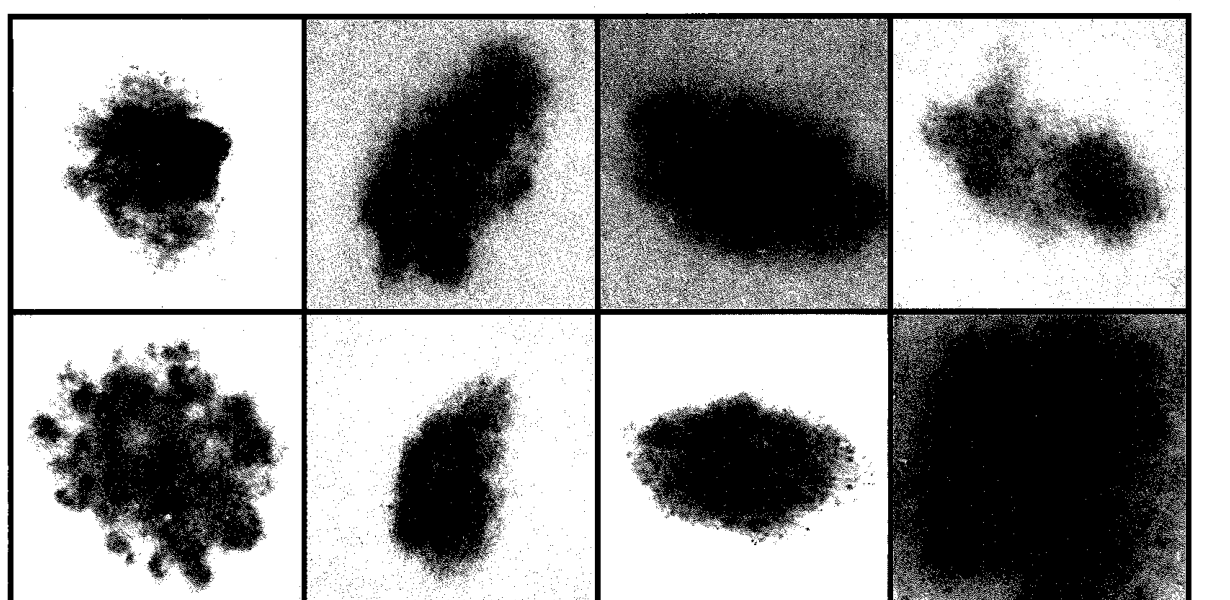
\includegraphics[width=0.85\textwidth]{ch01-fig1-1-skin-lesion.png}
  \caption{上面的一行图像是危险的恶性黑色素瘤，下面的一行图像是良性痣。未经专业训练的人很难区分这两类皮肤病变类型。}
  \label{figure:ch01-皮肤病变}
\end{figure}

\subsection{蛋白质结构预测}\label{subsection:ch01-蛋白质结构预测}

蛋白质常被称为生物体的基石。它们是由一个或多个氨基酸的长链组成的生物分子，蛋白质的特性则由22种不同类型的氨基酸序列所决定。当蛋白质在活细胞内合成后，就会折叠成复杂的三维结构，其行为和相互作用很大程度上取决于折叠的形态。

怎么根据氨基酸序列推导出蛋白质的三维结构呢？这是生物学界几十年来一直想攻克的基础性难题，但是进展甚微，直到深度学习技术带来了突破性进展。

蛋白质的三维结构可以通过X射线晶体学、低温电子显微镜或核磁共振光谱等实验技术进行测定。然而，这个过程通常非常耗时，而且对某些蛋白质来说，这种方法极具挑战性。例如，很难得到蛋白质的纯净样本，或者蛋白质的结构依赖于特定环境。相比之下，确定蛋白质的氨基酸序列的实验成本较低，产出较高。因此，如何直接从氨基酸序列预测蛋白质的三维结构引起广泛关注，这有助于更好地了解生物过程，以及用于新药研发等实际应用。我们可以以氨基酸序列为输入、以蛋白质的三维结构为输出来训练深度学习模型，其中的训练数据包含了已知的氨基酸序列和对应的蛋白质三维结构。因此，蛋白质结构预测也是监督学习的一个例子。经过训练的系统能够以新的氨基酸序列为输入，预测对应的蛋白质三维结构（Jumper et al., 2021）。\cref{figure:ch01-蛋白质结构}比较了一种蛋白质的预测三维结构和通过X射线晶体学获得的实际三维结构。

\begin{figure}[htbp]
  \centering
  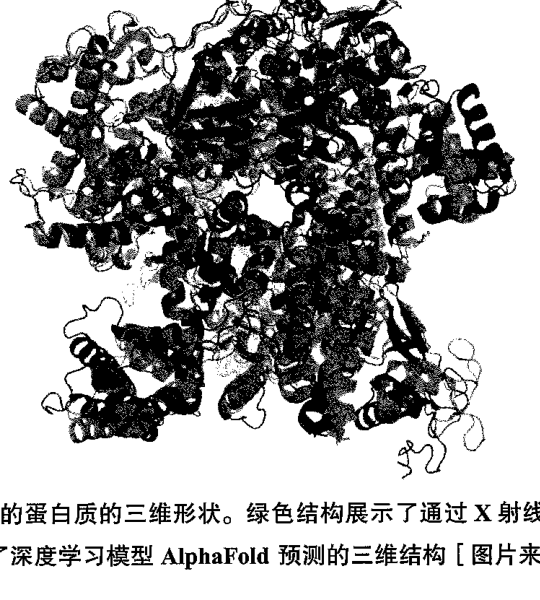
\includegraphics[width=0.5\textwidth]{ch01-fig1-2-protein-structure.png}
  \caption{一种名为T1044/6VR4的蛋白质的三维形状。绿色结构展示了通过X射线晶体学确定的真实三维结构，而叠加在上面的蓝色结构展示了深度学习模型AlphaFold预测的三维结构（图片来源于Jumper et al. (2021)，经许可使用）。}
  \label{figure:ch01-蛋白质结构}
\end{figure}

\subsection{图像合成}\label{subsection:ch01-图像合成}

在上面讨论的两个应用中，神经网络学会了将输入（皮肤图像或氨基酸序列）转换成输出（病变分类或蛋白质的三维结构）。现在我们来看一个不同的例子：训练数据是一组样本图像，训练后的神经网络能生成类似的新图像。与病变分类和蛋白质结构预测的例子不同，这些训练图像是没有标注的，这样的训练属于无监督学习（unsupervised learning）。\cref{figure:ch01-生成人脸}展示了一些由深度神经网络生成的合成图像，该深度神经网络是在拍摄于摄影棚单色背景下的人脸图像集上进行训练的。这些合成图像质量极高，很难将它们和真人照片区分开来。

这种模型可以生成与训练数据不同但又有类似统计特性的结果，所以被称为生成式模型（generative model）。这种方法的一个变体能根据输入的文本字符串（称为提示词，prompt）生成反映文本语义的图像（参见\cref{chapter:ch10-卷积网络}）。我们用生成式AI（generative AI）这个术语来描述那些能生成图像、视频、音频、文本、候选药物分子或其他形态信息的深度学习模型。

\begin{figure}[htbp]
  \centering
  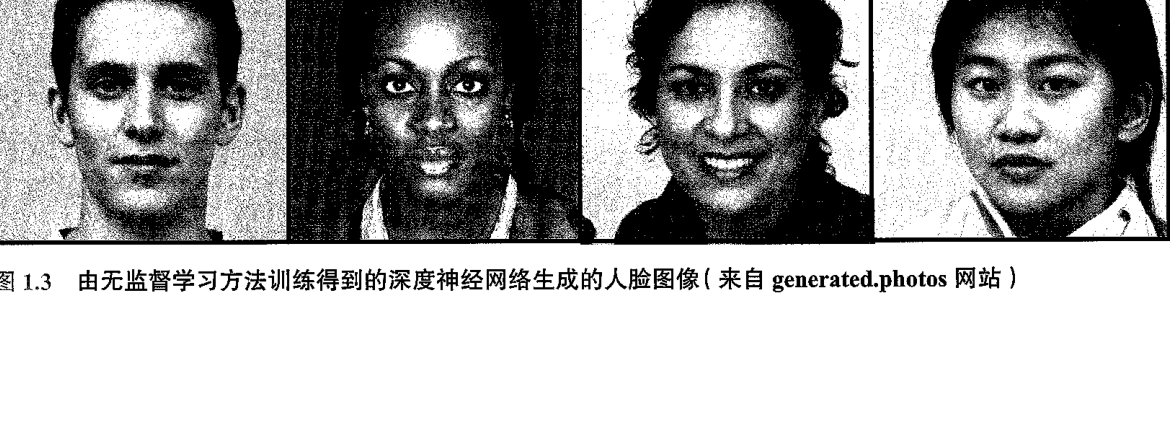
\includegraphics[width=0.85\textwidth]{ch01-fig1-3-generated-faces.png}
  \caption{由无监督学习方法训练得到的深度神经网络生成的人脸图像（来自generated.photos网站）。}
  \label{figure:ch01-生成人脸}
\end{figure}

\subsection{大语言模型}\label{subsection:ch01-大语言模型}

近年来，机器学习领域最重要的进展之一，是研发人员开发出了强大的模型来处理自然语言和类似程序代码这样的序列数据。大语言模型（Large Language Model, LLM）利用深度学习技术构建丰富的内部表征，捕捉语言的语义属性。有一类重要的大语言模型称为自回归（autoregressive）语言模型，它们能够输出语言，因此属于生成式AI的一种。这类模型以一个词序列作为输入，生成这个词序列最可能的下一个词，我们可以把末尾添加了新词的扩展序列再输入到模型中，让它生成后续的词，重复这个过程，就会得到越来越长的词序列。这样的模型还可以输出一个特殊的"停止"词，来表示文本生成的结束，这样就使得模型在输出一定长度的文本后停止。此时，用户可以在词序列的末尾添加自定义的词序列，然后将完整的词序列重新输入模型以触发生成后续的词。通过这种方式，人们就可以和神经网络对话了。

这类模型可以在大型文本数据集上通过提取训练对（training pair）进行训练。训练对的输入是随机选定的词序列，输出是已知的下一个词。这是自监督学习（self-supervised learning）的一个例子，在自监督学习中，模型学习从输入到输出映射函数，有标注的输出是从输入训练数据中自动获取的，无须进行另外的人工标注。这种方法能把多种来源的大量文本作为大型训练集，从而训练出超大规模神经网络。

一些专家认为，展现出非凡能力的大语言模型是通用人工智能的雏形（Bubeck et al., 2023），本书后面将详细讨论这类模型（参见\cref{chapter:ch12-transformer}）。接下来，我们给出一个基于GPT-4（OpenAI, 2023）的语言生成示例。GPT-4能够针对如下提示做出响应："请以莎士比亚戏剧风格，通过两个角色对话展开争论的方式证明素数有无穷多个"，如\cref{figure:ch01-gpt4素数证明}所示。

\end{document}